\chapter{評価スコアを推定するモデルの構築}
\thispagestyle{myheadings}

本章では,UTAU音源ライブラリに対して声質に対する評価スコアを付与するための機械学習モデルの概要と実装について述べる.
\ref{sec:utau}節では推論に用いるUTAU音源ライブラリとUTAU音源声質アンケートについて述べる.
\ref{sec:feature}節では使用する音声ファイルと音響特徴量,その抽出方法について述べる.
\ref{sec:model}節では評価スコアを推論する機械学習モデルの構築について述べ,\ref{sec:eval}節で構築したモデルの精度を評価する.

\section{UTAU音源ライブラリとUTAU音源声質アンケート}
\label{sec:utau}

本研究において探索対象とするUTAU音源ライブラリと,声質評価の基準として用いるUTAU音源声質アンケートについて説明する.
UTAU音源ライブラリは,無償で公開されている歌唱用音声合成ソフトウェアであるUTAU,およびその互換ソフトウェア上で使用できるライブラリであり,このライブラリを切り替えると実際に合成される音声を変更できる.
UTAU音源ライブラリは個人が作成・公開が可能で,ソフトと同じく無償で公開されているものが多い.
現在広く用いられている連続音方式であれば「あんああいあうあ」\cite{tatsu3shiki}といった形で複数の音素をできる限り一定の音程と音量になるように収録された肉声がwavファイルとして保存されいる.
UTAUは波形接続と呼ばれる手法を用いており,この音声データを切り貼りして歌声を合成し出力する.

UTAU音源声質アンケートはニコニコ大百科上で提言されたUTAU音源ライブラリに対してその声の特徴を評価するためのアンケート規格であり\cite{utausurvey},現在までにこの規格を用いて250種以上のUTAU音源ライブラリに対してアンケートが行われている.
このアンケートは表\ref{tab:survey}に示す7項目について,それぞれ1から7までの7段階評価で10件以上のアンケート調査を行い,その平均を評価値としている.

\begin{table}[htb]
  \centering
  \caption{UTAU音源声質アンケートの評価軸}
  \label{tab:survey}
  \begin{tabular}{c|cc}
    \hline
    評価軸 & 低い値の示す表現語 & 高い値の示す表現語 \\
    \hline
    声の性別 & 女性的 & 男性的 \\
    滑舌 & 舌足らず & はきはき \\
    特有性 & 素直 & 癖がある \\
    声の年齢 & 幼い & 大人びた \\
    透明感 & ノイジー & クリア \\
    声の強さ & 優しい & 力強い \\
    声の明度 & 暗い & 明るい \\
    \hline
  \end{tabular}
\end{table}

\section{特徴量の抽出}
\label{sec:feature}

UTAU音源ライブラリから推論に用いる音響特徴量を抽出する方法について述べる.
特徴量の抽出には,UTAU音源ライブラリから複数の音階で「あ」「い」「う」「え」「お」「ん」と発声した音声をライブラリ中の音声ファイルを直接操作して作成し,利用する.
五母音と子音「ん」は連続して発声のできる音素であり,安定して音声の特徴を抽出できる.
音声ファイルの操作時には,この範囲はUTAU上で音声が合成される際母音を伸ばすために用いる範囲である,子音部とブランクとしてライブラリに指定されるタイミング間の音声を利用した.
図\ref{fig:waveform}に「あ」を発生している音声ファイルの波形とスペクトログラム,ライブラリに指定されるタイミングの例を示す.
この図はUTAU互換ソフトウェアであるOpenUTAUからキャプチャしたものである.
波形上に塗られた赤いエリアの終わりが子音部,右端の青色の縦線がブランクとして指定されたタイミングを示す.
この範囲は音声の発声始めや次の音素の発音に移る部分を含まないため,音声波形とスペクトログラムの形状が安定している.
安定した声が収録されているため音声の特徴を抽出する上で適していると考えた.
音階はA3,D4,G4,C5,F5の5音階を用いる.
複数の音階を用いる特徴量の数を増加させるほか,音声の音域による特徴への影響などを反映できると考えられる.
複数音階の音声の生成には,ライブラリで音階ごとに指定される適切な音声ファイルからピッチシフトを行い生成した.

\begin{figure}[h]
  \centering
  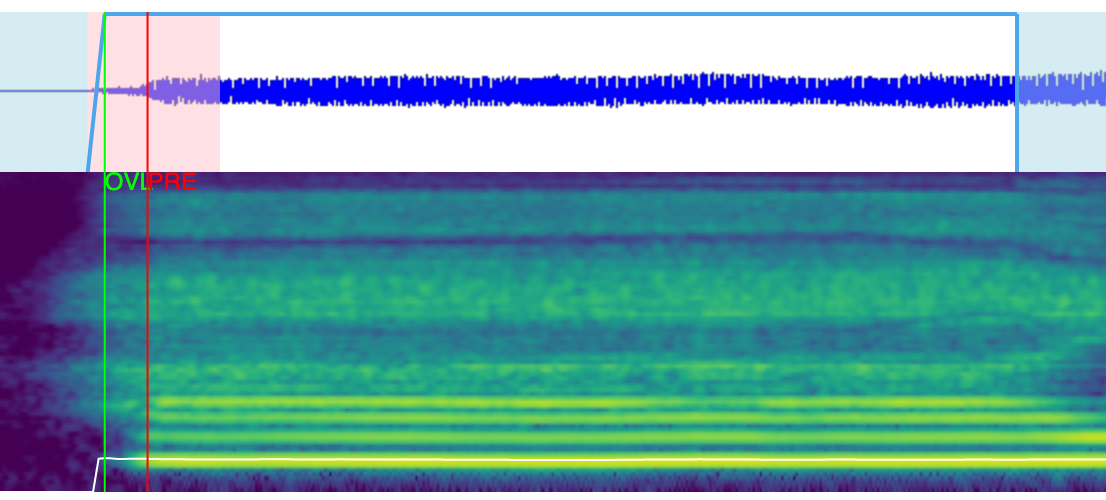
\includegraphics[width=0.9\linewidth]{fig/eve_a.png}
  \caption{音声ファイルの波形とスペクトログラム,ライブラリに指定されるタイミング}
  \label{fig:waveform}
\end{figure}

実際に用いる特徴量としては,MFCC,ZCR,F1〜F4の周波数を採用した.
Pythonライブラリであるlibrosaを用いて各音階と音素ごとにこれらの特徴量を抽出し,評価スコアの推論に用いた.
以下にそれぞれの特徴量について説明する.

MFCCはメル周波数ケプストラム係数の略で,音声の周波数成分を人間の聴覚特性に基づいて変換した数列である.
音声信号に対してフーリエ変換を適用して得られる周波数スペクトルを,人間の聴覚特性に合わせて変換(メルスケール変換)し,さらに対数変換と離散コサイン変換を適用して得られる.
周波数スペクトルと比較してMFCCは聴覚特性に合わせた特徴量を持つため,人間からの聞こえ方の特徴を反映しているとされ,音声の声質に関連すると考えられるため採用した.
本研究では生成した音声からMFCCを64次元まで取得し用いる.

ZCRは音声の波形が0を交差する頻度を表す指標であり,音声信号の時間軸上で波形が正から負,または負から正に変化する回数を示す.
高い音声ほど周波数が高くなり波形の変化が多くなることから,ZCRも高くなるほか,摩擦音のような雑音成分が多い音声でもZCRは高くなる.
音声の声高を固定した今回の音声であれば,音声の透明感などに関連する指標として扱えると考え採用した.

フォルマントは周波数スペクトルのピークの周波数であり,周波数の低いものから順にF1,F2,と言った具合に呼ばれる.
フォルマントは声質や音素の音色に大きく関係する特徴量で特に母音の認識に重要とされており,音声の母音によってそのフォルマント周波数には一定の傾向がある.
粕谷らの研究によれば,同じ母音のフォルマント周波数でも話者の年齢や性別によって変化があり\cite{formant},声の性別感や年齢感に影響があると考えられる.

\section{モデルの構築}
\label{sec:model}

モデルの構築にはPythonライブラリであるPyCaretを用いた.
PyCaretは機械学習モデルの作成を簡略化するためのライブラリであり,データの前処理からモデルの選定,評価までを一連の流れで行える.
各評価スコアを推論の目標として与え,先述の特徴量から評価スコアを推定するモデルを評価スコアの7軸それぞれについて別々に作成した.

UTAU音源声質アンケートの結果はExcelファイルとして提供されている.
このファイルに記載されている240種のUTAU音源ライブラリのうち,現在でもダウンロードが可能であり,必要な音素が収録されていて,かつ利用規約上で研究目的を含む機械学習用途での利用が禁止されていない168ライブラリを学習対象とした.
データセットは学習データとテストデータに分割し,ランダムに選択した30\%をテストデータ,残りの70\%を学習データとして使用した.

7つの評価軸それぞれについてPyCaretで選択できるモデルごとの推定精度を比較した結果,全体的に精度の優れていたAdaBoost Regressorを選択した.
学習モデルを選択する際は,ランダムフォレストなどの離散モデルではなく線形回帰などの連続モデルの中から選択した.
これは連続量である特徴量から連続量である評価スコアを推定するため一定の値のみを推定結果に取る離散モデルよりも適していると考えたほか,予備実験において離散モデルでの学習時に過学習の傾向が頻繁に見られたためである.

\section{結果の評価}
\label{sec:eval}

構築したモデルによる推論の精度を評価するため,テストデータに対して推論を行い得た値と実際のアンケートによって得られた値を比較する.
テストデータは先述の通り学習データから各評価軸ごとにランダムに選ばれたデータであり,対象とした168ライブラリの3割にあたる51ライブラリを用いた.

図\ref{tab:score_box}では,横軸は評価軸を,縦軸はテストデータにおける実際の値と推測された値との誤差の二乗平均平方根(Root Mean Square Error: RMSE),エラーバーは誤差の標準偏差を示している.
RMSEは実際の値と推測された値の差を二乗して平均を取った後に平方根を求めたもので,数値予測モデルの精度を評価する際によく用いられる指標である.
結果を見ると,RMSEの最も小さい「滑舌」の軸では0.72,最も大きい「声の性別」の軸では1.27を示しており,評価軸ごとに大きな差は見られなかった.
RMSEは0に近いほど予測精度が高いことを示し,評価スコアが1から7までの7段階であることを考慮すると,全体的に中程度の精度が得られたと言える.
これらの結果は先行研究\cite{dnn}での報告値と近い値であり,音響特徴量を用いた機械学習モデルとして一定の妥当性を示すことができた.
また,エラーバーの大きさから,評価軸によって予測の安定性に差があることも確認できる.

\begin{figure}[h]
  \centering
  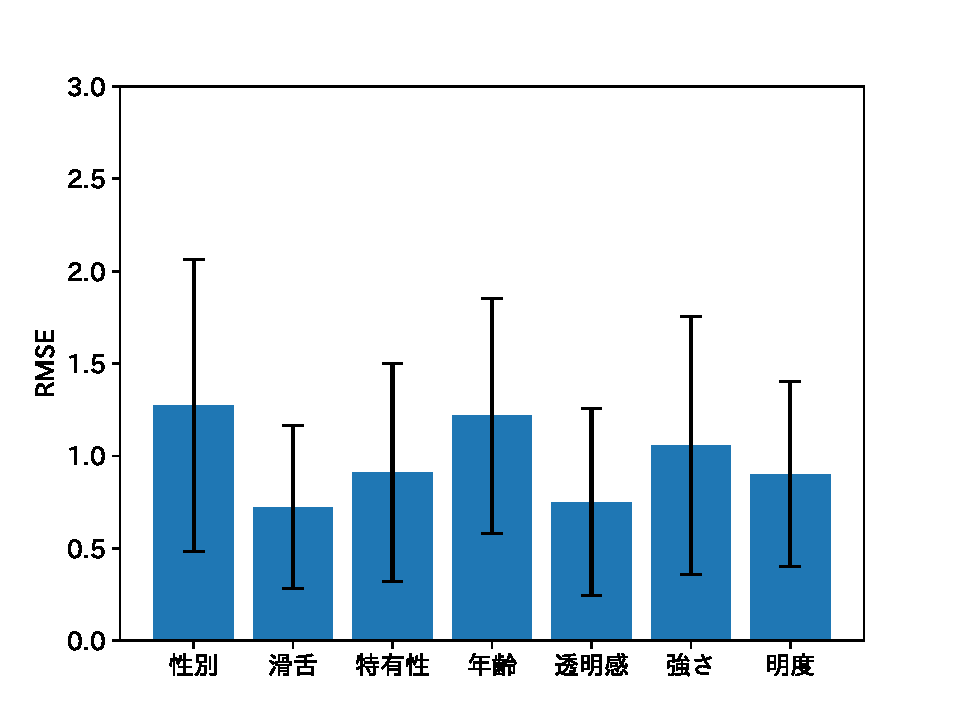
\includegraphics[width=\linewidth]{fig/rmse.pdf}
  \caption{テストデータとの誤差の二乗平均平方根}
  \label{tab:score_box}
\end{figure}

図\ref{tab:score_coor}では,横軸は評価軸を,縦軸はテストデータにおける実際の値と推測された値との相関係数を示している.
相関係数は一般に0.7以上であればデータ間に強い相関が,0.4以上であればある程度の相関があるとされ,実際の値と推測された値における相関が強いほど推論の精度が高いと言える.
結果を見ると,最も低い「声の年齢」は0.20とかなり低いものの,他の評価軸では0.49から0.66程度,最も高い「声の強さ」では0.66と,ある程度の相関が見られた.

\begin{figure}[h]
  \centering
  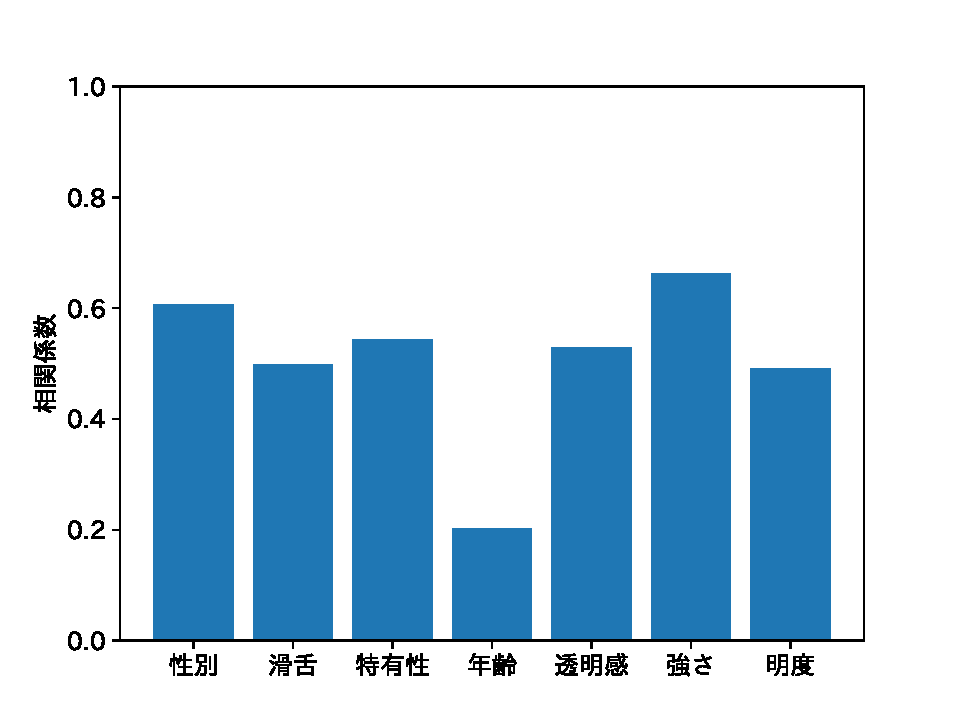
\includegraphics[width=\linewidth]{fig/coorpdf.pdf}
  \caption{テストデータとの相関係数}
  \label{tab:score_coor}
\end{figure}

7つの評価軸ごとの予測された値と実際の値との散布図を図\ref{fig:scatters}に示す.
図を見ると,相関係数の高かった「声の強さ」は右肩上がりの傾向が見られ相関の存在が分かる一方で,最も低かった「声の年齢」では点が縦に長く分布しているのが分かる.
これは相関が弱いことに加え,実際の値はスコア範囲中に広く分布しているにも関わらず,予測された値がおおよそ3〜5と範囲の中央に偏っていることを表している.
このような傾向は程度の差はあるものの他の評価軸でも見られ,精度を下げてる一因となっている.

\begin{figure}[htb]
  \centering
  \subcaptionbox{声の性別}{
  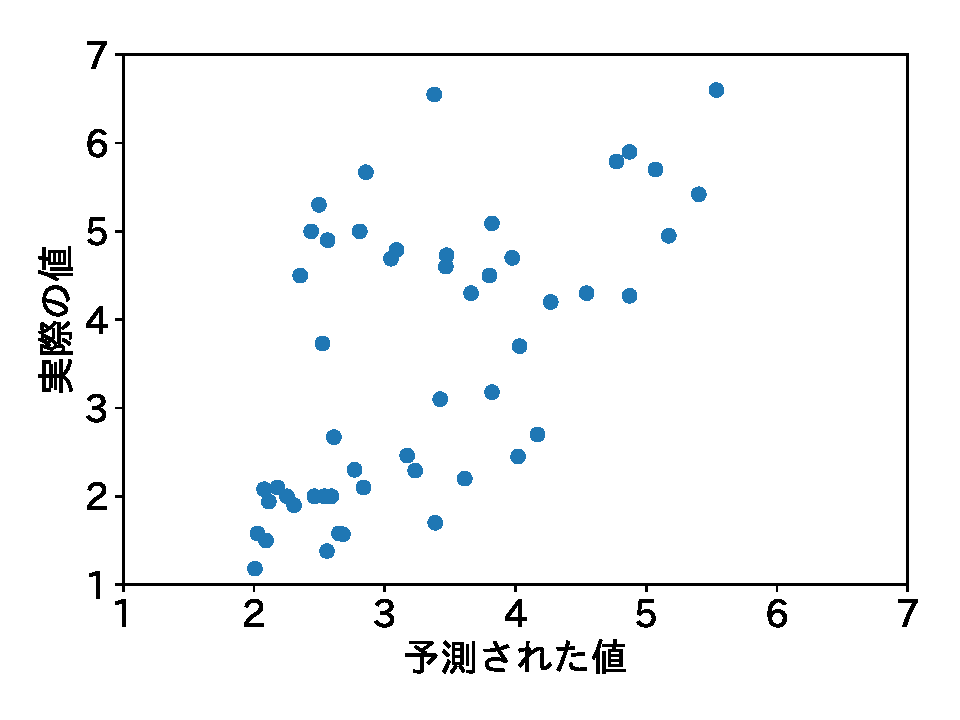
\includegraphics[width=0.4\linewidth]{fig/scatter/0.pdf}}
  \hspace{3mm}
  \subcaptionbox{滑舌}{
  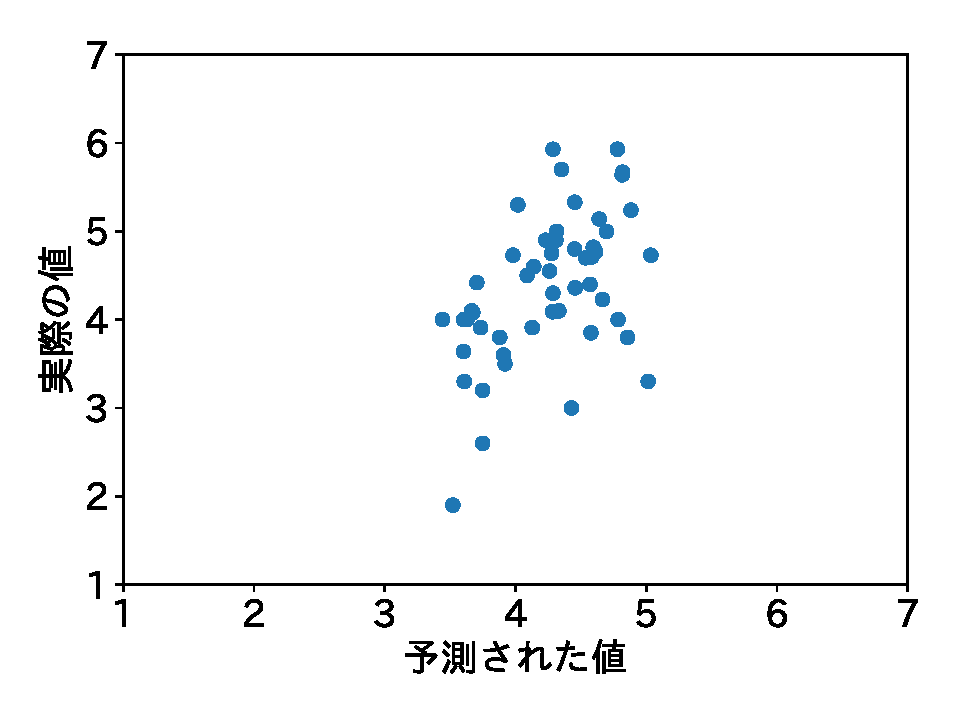
\includegraphics[width=0.4\linewidth]{fig/scatter/1.pdf}}
  \vspace{3mm}
  \subcaptionbox{特有性}{
  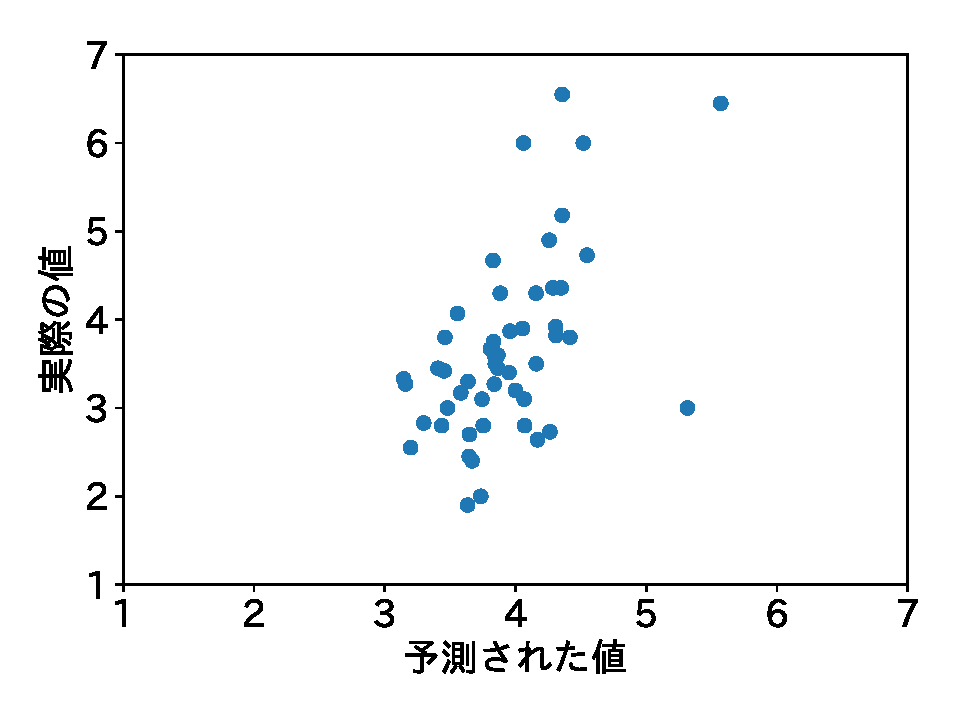
\includegraphics[width=0.4\linewidth]{fig/scatter/2.pdf}}
  \hspace{3mm}
  \subcaptionbox{声の年齢}{
  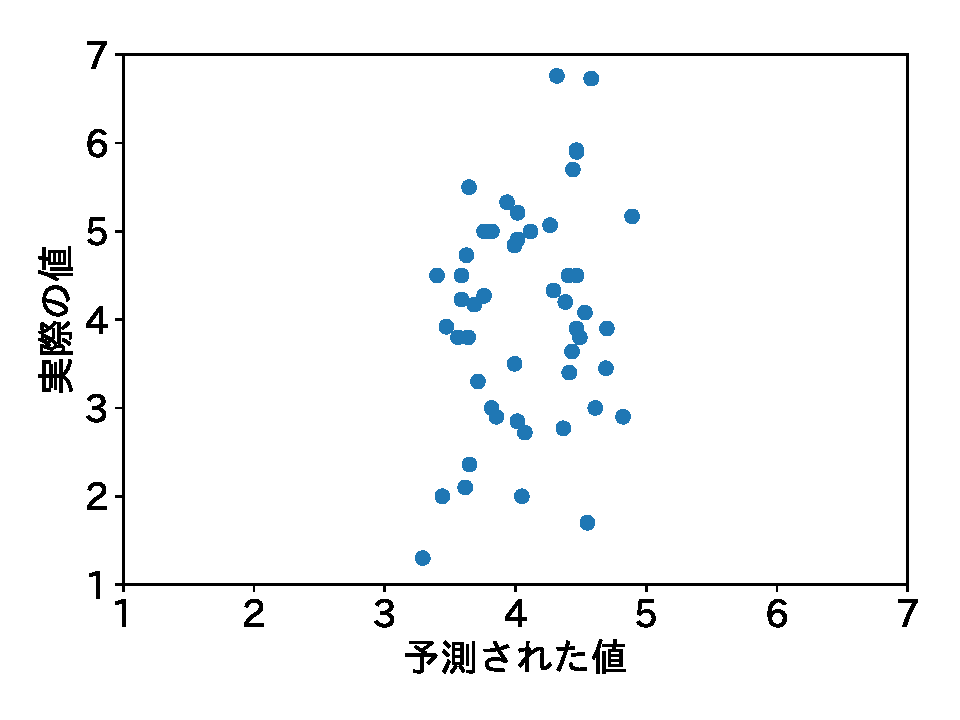
\includegraphics[width=0.4\linewidth]{fig/scatter/3.pdf}}
  \vspace{3mm}
  \subcaptionbox{透明感}{
  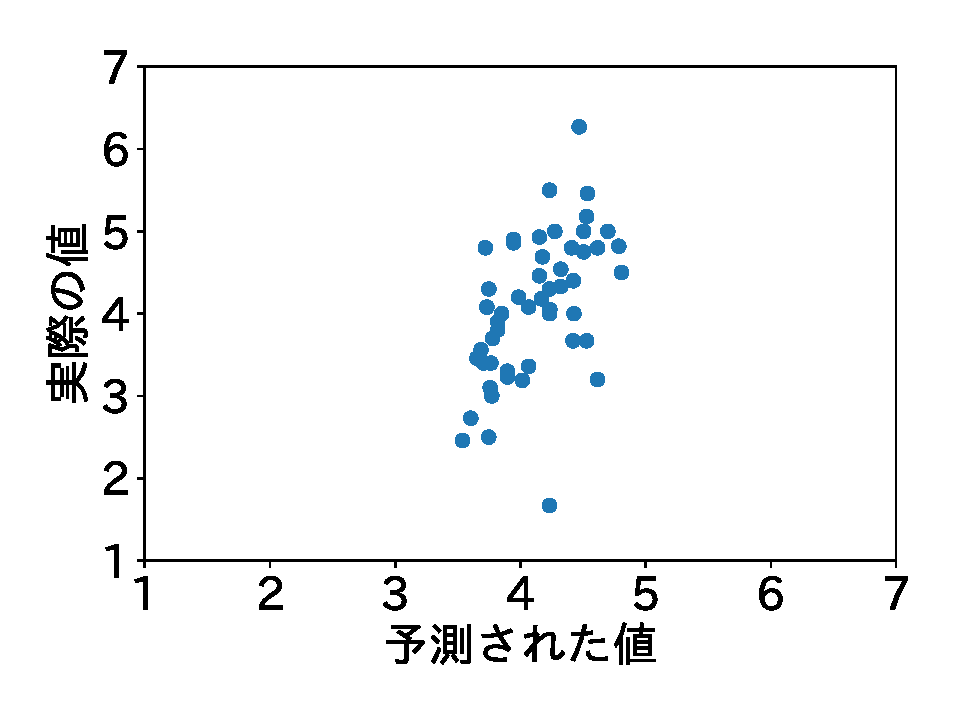
\includegraphics[width=0.4\linewidth]{fig/scatter/4.pdf}}
  \hspace{3mm}
  \subcaptionbox{声の強さ}{
  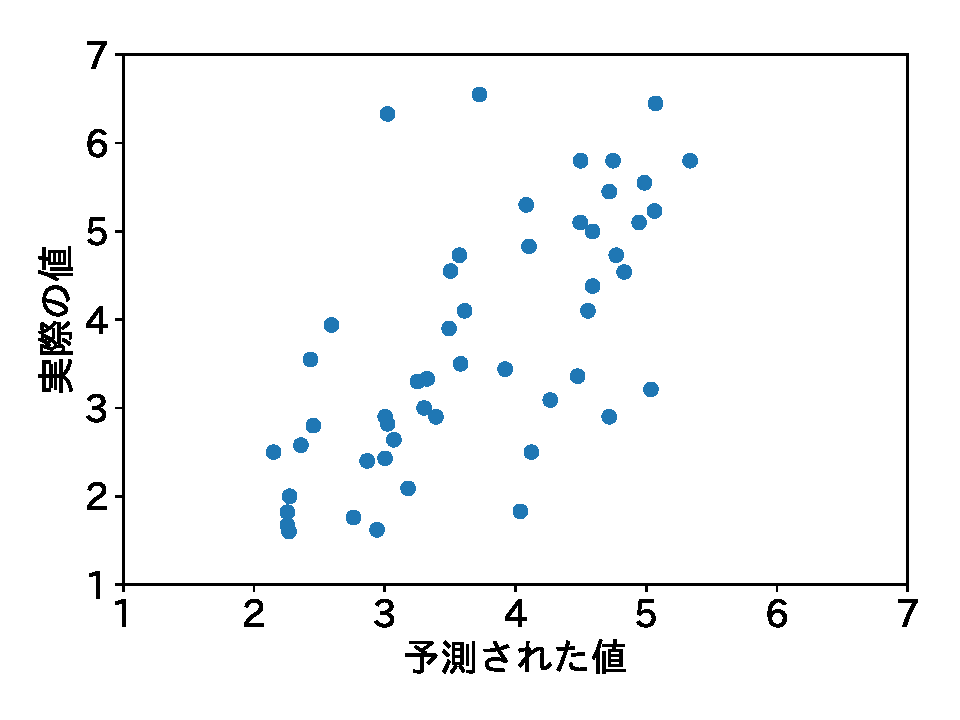
\includegraphics[width=0.4\linewidth]{fig/scatter/5.pdf}}
  \vspace{3mm}
  \subcaptionbox{声の明度}{
  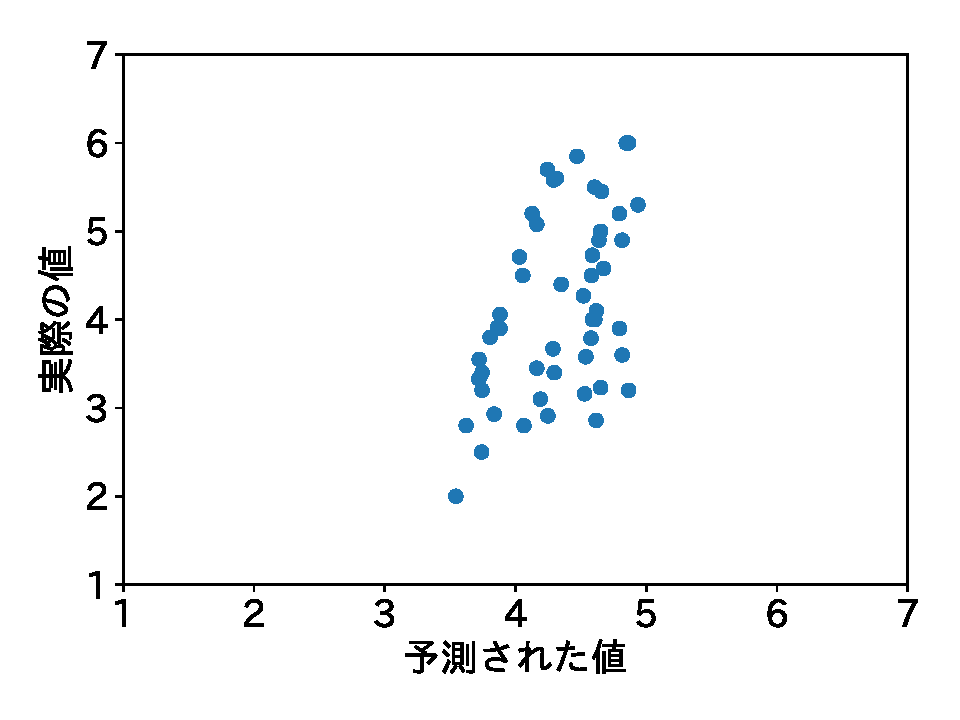
\includegraphics[width=0.4\linewidth]{fig/scatter/6.pdf}}
  \caption{実際の値と推測された値の散布図}
  \label{fig:scatters}
\end{figure}

予測値が中央に偏る現象について,一般にはデータの偏りやモデルの過学習,特徴量の不足などが要因とされている.
学習データを確認したが,テストデータのスコア分布からも分かるように,実際のスコアは広く分布しておりスコアの偏りは認められなかったほか,モデルの過学習についてもそのような傾向は見られなかった.
一方で,今回用いた音声特徴量が声質の印象に対し十分でなかった可能性は十分に考えられる.
主に母音に対して音階ごとに別々の特徴量を抽出したが,本研究で用いなかった子音にまつわる特徴量や音素間の遷移の特徴などの特徴量も声の印象に影響していると考えられる.
そのほか先行研究\cite{dnn}では機械学習の手法としてディープラーニングのモデルが採用されていたように,学習手法も複数のものが考えられる.
様々な手法を試し,より適したものに変えることで性能向上の余地があると考えられる.

% Local Variables:
% mode: japanese-LaTeX
% TeX-master: "root"
% End:
